\documentclass{beamer}
\setbeameroption{show notes}
\newcommand{\irptitle}{Remaining Anonymous when using the Bitcoin Protocol}
\usepackage[style=ieee]{biblatex}
\addbibresource{i-d.bib}
\addbibresource{report.bib}
\addbibresource{rfc.bib}

\newcommand\irptopic{Bitcoin}
\newcommand\irpauthor{Thomas A. Grainger}

\newcommand\MYhyperrefoptions{bookmarks=true,bookmarksnumbered=true,
pdfpagemode={UseOutlines},plainpages=false,pdfpagelabels=true,
hidelinks,
pdftitle={\irptitle},%<!CHANGE!
pdfsubject={\irptopic},%<!CHANGE!
pdfauthor={Thomas A. Grainger},%<!CHANGE!
pdfkeywords={Bitcoin, Anonymity, Cryptography, crypto-currencies, Peer to Peer}}
\renewcommand{\biblabelsep}{2em}
\renewcommand{\bibitemsep}{0.2ex}
\renewcommand*{\bibfont}{\tiny}

\usetheme{Madrid} % My favorite!
%\usetheme{Boadilla} % Pretty neat, soft color.
%\usetheme{default}
%\usetheme{Warsaw}
%\usetheme{Bergen} % This template has nagivation on the left
%\usetheme{Frankfurt} % Similar to the default 
%with an extra region at the top.
%\usecolortheme{seahorse} % Simple and clean template
%\usetheme{Darmstadt} % not so good
% Uncomment the following line if you want %
% page numbers and using Warsaw theme%
% \setbeamertemplate{footline}[page number]
%\setbeamercovered{transparent}
\setbeamercovered{invisible}
% To remove the navigation symbols from 
% the bottom of slides%
\setbeamertemplate{navigation symbols}{} 
%
\usepackage{graphicx}
%\usepackage{bm}         % For typesetting bold math (not \mathbold)
%\logo{\includegraphics[height=0.6cm]{yourlogo.eps}}
%
\title[\irptopic]{\irptitle}
\author{\irpauthor}
\institute[U of S]
{
University of Southampton \\
\medskip
{\emph{t.grainger@ecs.soton.ac.uk}}
}
\date{\today}
% \today will show current date. 
% Alternatively, you can specify a date.
%
\begin{document}
%
\begin{frame}
\titlepage
\note{Hi, My name is Thomas Grainger, and I'll be talking to you about  Bitcoin: the decentralized digital currency.}
\end{frame}
%
\begin{frame}
\frametitle{Introduction}
\begin{figure}[h!]
    \centering
    \includegraphics[width=0.8\columnwidth]{img/dyn/price}
    \caption{A chart showing the price of Bitcoin over time in USD (source \href{http://bitcoincharts.com/}{bitcoin charts})}
    \label{fig:blockchain}
\end{figure}
\note{As you can see from the latest price charts bitcoins do have, although extremely volatile, a `real world' value.}
\end{frame}
%TODO: TABLE OF CONTENTS?
\begin{frame}
\frametitle{Existing Systems}
\begin{description}
    \note{So, first of all - I'm going to talk to you about the existing systems that helped lead to Bitcoin}
    \item[Central Banking Authorities]\hfill \\
        SEPA and PayPal~\cite{paypal}.\note{These fully central systems, such as PayPal, or SEPA handle transactions by debiting one user account and crediting another}
    \item[Unique Token]\hfill \\
        NetCash~\cite{netcash}.\note{In NetCash the user and central authority agree on a unique token. To transfer value a user sends a token to another user. Receiving users send the token to the exchange, to be swapped for a new spendable token invalidating the original token}
    \item[Blind-signing]\hfill \\
        Chaumian e-Cash\cite{chaum}.\note{Chaumian e-Cash uses blind signatures created by a central service. These signatures can be verified by the central server without knowing who originally requested them.}
    \item[Digital Signature Chain]\hfill \\
        B-Money\cite{b-money}. \note{In B-Money transaction messages are created using public key cryptography\ldots}
\end{description}
\end{frame}
%

\begin{frame}
\frametitle{Existing Systems}
\framesubtitle{B-Money}
\note{\ldots and the chain of digital signatures can be traced back to the original creation of value.}
\begin{figure}[h!]
    \centering
    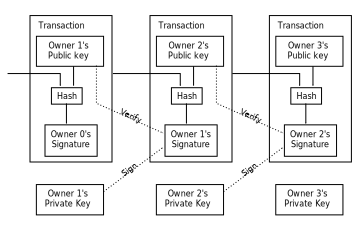
\includegraphics[width=0.8\columnwidth]{img/Bitcoin_Transaction_Visual}
    \caption{A chain of digital signatures representing value transfer.
    (source \protect\cite{satoshi})}
    \label{fig:chain-spend}
\end{figure}
\note{However, without a ``synchronous and unjammable anonymous broadcast channel'' it is impossible to tell if one user has signed away more than his or her share of money, a double spend}
\end{frame}

\begin{frame}
\frametitle{The Bitcoin Protocol}
The Bitcoin block chain is a concrete implementation of B-Money\\\note{The Bitcoin protocol and client software provides a concrete implementation of an altered version of the original B-Money proposal.}
But it uses a block chain.\note{In that it uses a block chain instead of a ``synchronous and unjammable anonymous broadcast channel''}
\begin{block}
{Blocks\ldots}
\begin{itemize}
\item contain the latest transactions
\item refer to the previous block in the chain by hash value
\item must meet a ``proof-of-work'' requirement\note{This proof of work is calculated by repeatedly hashing blocks until a low enough SHA256 value is discovered}
\end{itemize}
\end{block}
\end{frame}

\begin{frame}
\frametitle{The Bitcoin Protocol}
\framesubtitle{The block chain}
\begin{figure}[h!]
    \centering
    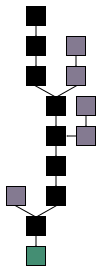
\includegraphics[angle=-90,totalwidth=0.8\columnwidth]{img/Blockchain}
    \caption{A diagram showing invalid blocks (grey) being invalidated by a block chain with greater totally difficulty (black). (based on work from \href{http://theymos.com/}{theymos})}
    \label{fig:blockchain}
\end{figure}
\note{This means to replace a block in the chain all later blocks must also be recreated, and thus all of their proof of work's need to be recreated. A bit like a `git rebase' except trillions of hashes must be calculated for each block}
\end{frame}

\begin{frame}
\frametitle{The Bitcoin Protocol}
\framesubtitle{Hash Power}
\begin{figure}[h!]
    \centering
    \includegraphics[width=0.8\columnwidth]{img/dyn/speed-lin-ever.png}
    \caption{A chart showing the total hash power of the Bitcoin network (source \href{http://bitcoin.sipa.be/speed-lin-ever.png}{SIPA})}
    \label{fig:blockchain}
\end{figure}
\note{*Point out the various peaks: The first bubble, The second bubble and ASICs}
\end{frame}

\begin{frame}
\frametitle{De-Anonymization Techniques}
\note{Because all transactions must be broadcast publicly, the Bitcoin client software uses hundreds of different keys as pseudonyms in a wallet.}
Heuristics can be used to contract the ``transaction network'' into a ``user network''.
\begin{description}
\item[Multi-Input Transactions] If a user cannot fulfill the value of a transaction by spending a  single previous output, the client will combine multiple inputs\cite{reid-anon}.
\item[Change Addresses] Because each output must be redeemed in it's entirety transactions of values smaller than the smallest output available to a wallet, the Bitcoin client uses ``change addresses'' so as to retain the remaining value.

Once contracted any address in a group, can be used to identify that whole group.
\note{Unfortunately, by downloading a copy of the transaction data and using some heuristics, it is possible to group keys back into a single wallet}
\end{description}
\end{frame}

\begin{frame}
\frametitle{De-Anonymization Techniques}
\begin{figure}[h!]
    \centering
    \includegraphics[width=0.8\columnwidth]{img/group_addresses}
    \caption{Two users send money to $k_{SR}$. Under the Multi-Input  heuristic $k_{a1}, k_{a2} and k_{a3}$ and $k_{b1}, k_{b2}$ are contracted into  some user $a$ and some user $b$. Under the change address heuristic  $k_{a4}$ and $k_{b3}$ are also contracted into user $a$ and user $b$  respectively. }
    \label{fig:blockchain}
    \note{As you can see it is clear that , under these heuristics, the keys in the red square and blue square can be grouped}
\end{figure}
\end{frame}


\begin{frame}
\frametitle{Anonymization Techniques}
\begin{description}
\note{Fortunately a few possibilities exist to remain hidden.}
\item[Fully Trusted Mixing]
A mixing service accepts Bitcoin transactions and automatically sends a new transaction to a newly generated Bitcoin address.
\item[ZeroCoin]
Uses a zero knowledge proof (ZKP) that only proves knowledge of: a Zerocoin in the block chain. The actual serial number used to generate it\cite{zerocoin}.
\item[In-Protocol Mixing]
Groups of users cooperate to create transactions that appear to link their wallets.

\note{Describe the bullets}
\end{description}
\end{frame}

\begin{frame}
\frametitle{Anonymization Techniques}
\note{I'm now going to show you how ZeroCoin works, I'm not going to explain the content on these slides \ldots}
\framesubtitle{ZeroCoin 1}
To spend a ZeroCoin (ZC), given all ZCs in the block chain ${C_1, C_2,\dots,C_N}$, prove knowledge of $C_i$ such that:

\begin{equation}
    (C_i = C_1) \vee (C_i=C_2) \vee \dots \vee (C_i=C_N)
\end{equation}

ZC uses a one-way public accumulator with an efficient ZKP that accumulates ${C_1, C_2,\dots,C_N}$ to produce some $A$, such that it's possible to prove knowledge of a witness s.t. $C_i \in inputs(A)$~\cite{one-way-accumulators}.

A Zerocoin $C_{i}$ is created using serial number $S$ in the group $Z(N)$ using a Peterson commitment, equation~\ref{eqn:zq-create}, repeated until $C_i$ is prime.

\begin{equation}\label{eqn:zq-create}
C_{i}=g^Sh^r, C_i \in \mathbb(P)
\end{equation}
\end{frame}

\begin{frame}
\frametitle{Anonymization Techniques}
\framesubtitle{ZeroCoin 2}
An accumulator $A$ can be created from the asserted ZCs.  Adding to the accumulator is trivial, $A' = A*u^{C_i}$.

\begin{subequations}
    \begin{align}\label{eqn:zkp}
        N &= p \cdot q, u \in QR_{N}(u\neq1)\\
        A &= u^{C_1, C_2,\dots,C_N}\\
        w_i &=  u^{C_1, C_2,\cdots C_{i-1}, C_{i+1}, \dots ,C_N}
    \end{align}
\end{subequations}

Where $N$ is the product of two permanently private prime numbers - these primes are generated once, multiplied to derive $N$ then are permanently destroyed.
\note{\ldots because it involves some funky use of cryptography, such as Zero Knowledge Proofs, and you'd need to understand group theory and how RSA works.}
\end{frame}


\begin{frame}
\frametitle{References}
\footnotesize{
\printbibliography
}
\end{frame}
 
\begin{frame}
\centerline{The End}
\end{frame}
% End of slides
\end{document} 